\subsection{Norte América}

En esta instancia de experimentaci'on vamos a analizar las rutas a la universidad de UNAM, ubicada en Mexico, utilizando la direcci'on \textit{unam.edu}. 

\begin{tabular}{ |p{1cm}||p{3cm}|p{2cm}|p{2cm}|p{1.5cm}|  }
 \hline
 \multicolumn{5}{|c|}{Traceroute a UNAM} \\
 \hline
 \textit{TTL} & \textit{IP}  & \textit{RTT} & $\delta$\textit{RTT} & Outlier? \\
 \hline
1    &    192.168.1.1    &     2.43 ms      &     -           &     \\               
2    &    Sin respuesta              &    -             &    -           &          \\                  
3     &   Sin respuesta              &    -            &     -         &        \\               
4    &    Sin respuesta               &    -            &     -          &        \\                   
5    &    Sin respuesta                &   -            &     -          &        \\                
6     &   200.89.161.85   &    19.59 ms     &     17.17 ms   &        \\              
7     &   200.89.165.197  &    20.53 ms     &     0.94 ms   &        \\            
8    &    200.89.165.222  &    22.96 ms     &     2.43 ms   &      \\               
9    &    Sin respuesta               &    -            &     -         &         \\                 
10   &    64.215.103.74    &   155.34 ms     &    132.38 ms  &  Outlier  \\    
11   &    159.63.49.142    &   192.17 ms    &     36.84 ms    &           \\              
12   &    201.140.112.97   &   184.71 ms    &     -         &           \\                
13   &    201.148.69.177   &   193.2 ms     &     1.03 ms         &      \\                    
14   &    132.247.237.217  &   184.7 ms      &    -         &           \\                 
15   &    132.247.237.189  &   183.25 ms    &     -         &          \\                  
16    &   132.247.70.37    &   176.05 ms     &    -        &       \\   
 \hline
\end{tabular}

\smallskip
    
\begin{figure}[H]
\centering
\caption{UNAM delta RTTs y ZRTT}
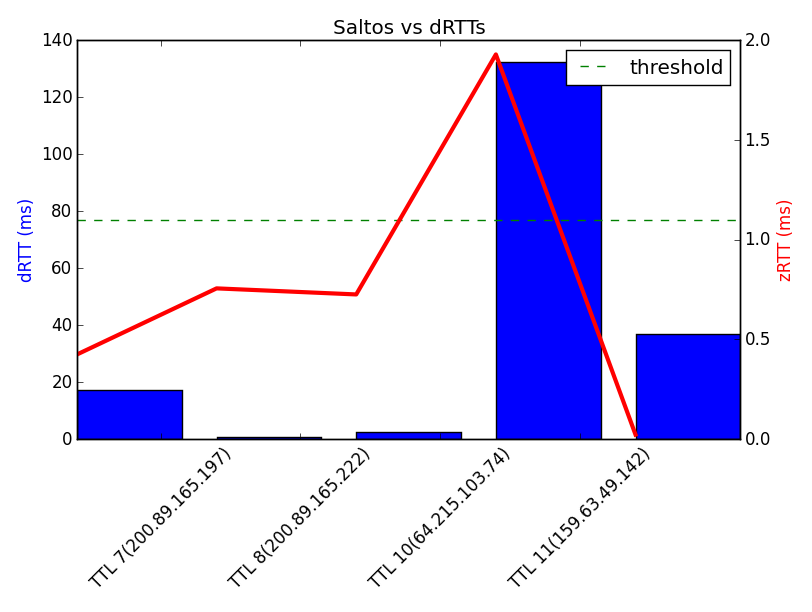
\includegraphics[width=0.55\textwidth]{modules/unam_rtts_2}
 \label{fig:unam_rtts_2}
\end{figure}

\begin{figure}[H]
\centering
\caption{UNAM RTTs por salto}
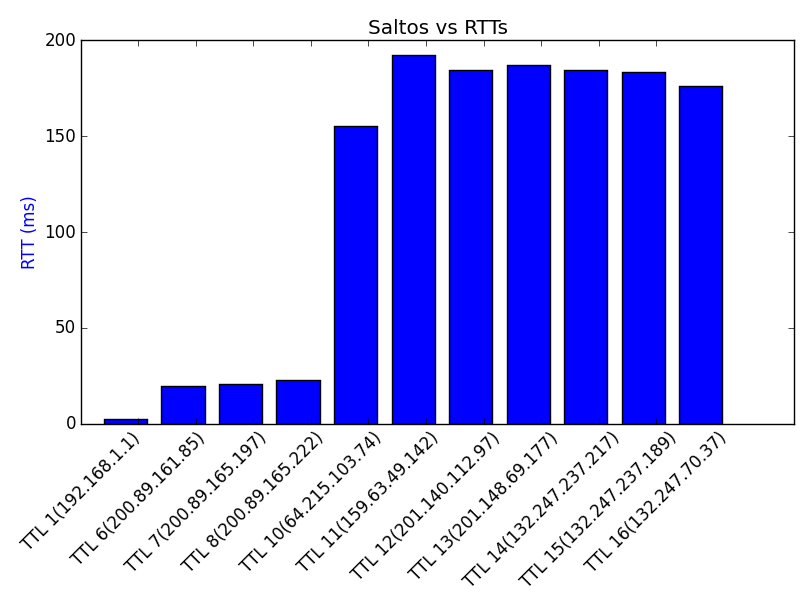
\includegraphics[width=0.55\textwidth]{modules/unam_rtts_1}
 \label{fig:unam_rtts}
\end{figure}

Mencionar que pasa por USA
\begin{figure}[H]
\centering
\caption{Ruta a UNAM}
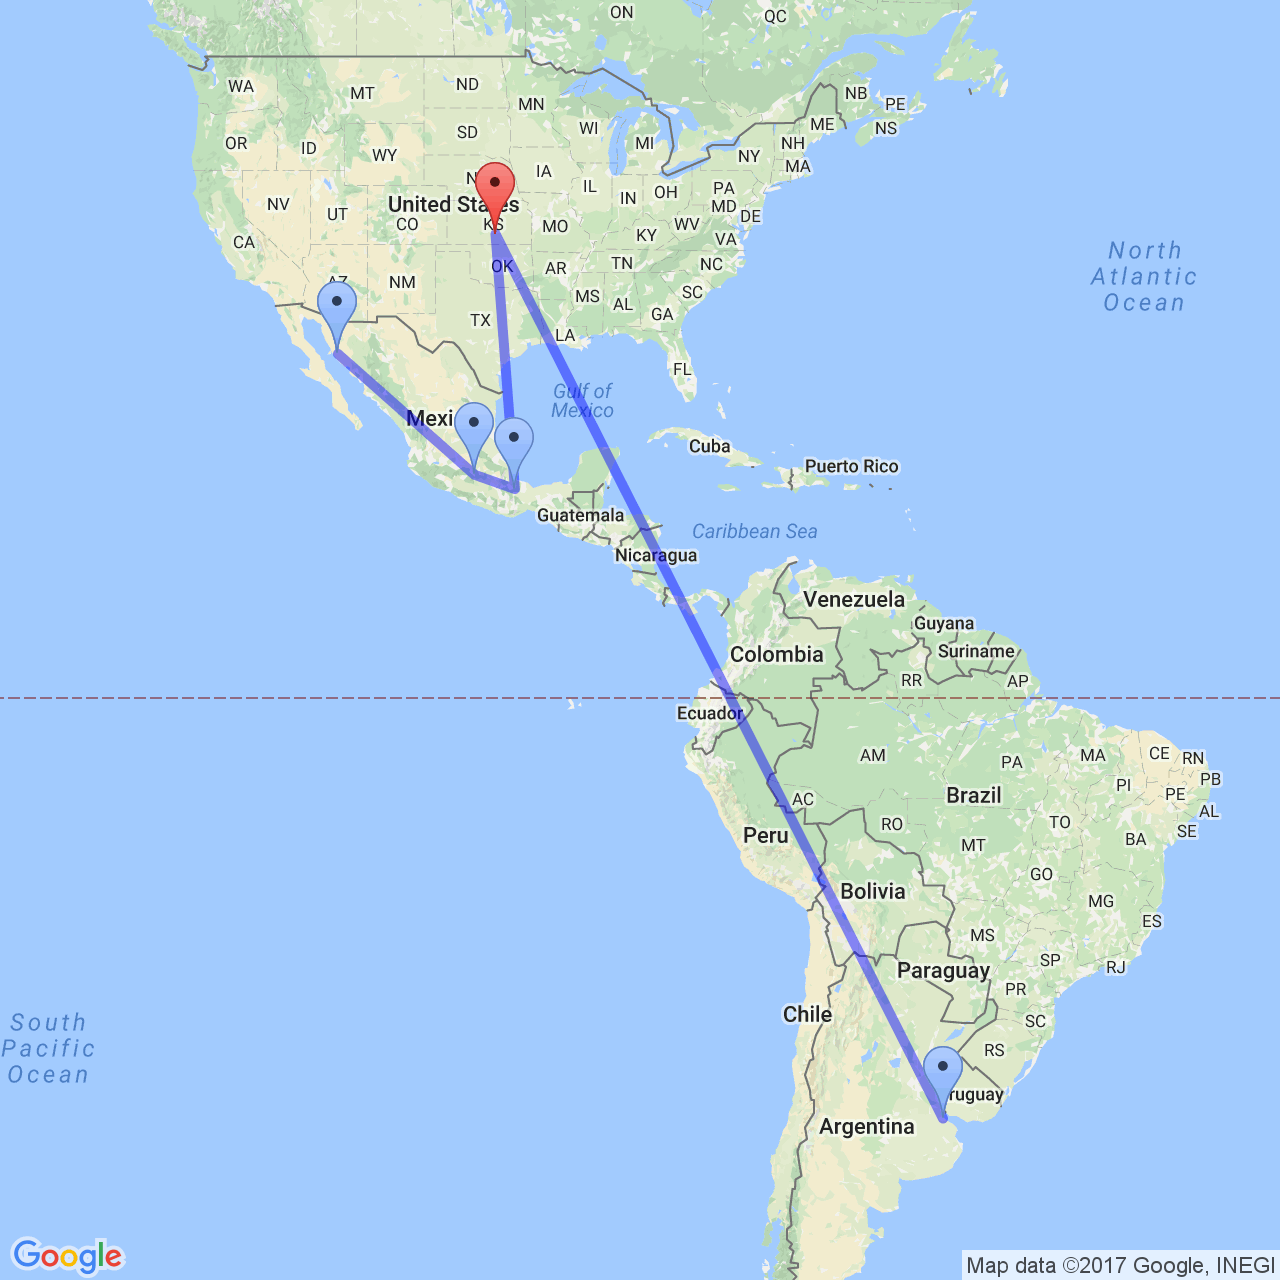
\includegraphics[width=0.55\textwidth]{modules/unam_path_1}
 \label{fig:ruta_unam_1}
\end{figure}

LPM UNAM no queda en el desierto de sonora, geolocation fallo
\begin{figure}[H]
\centering
\caption{Ruta en Mexico}
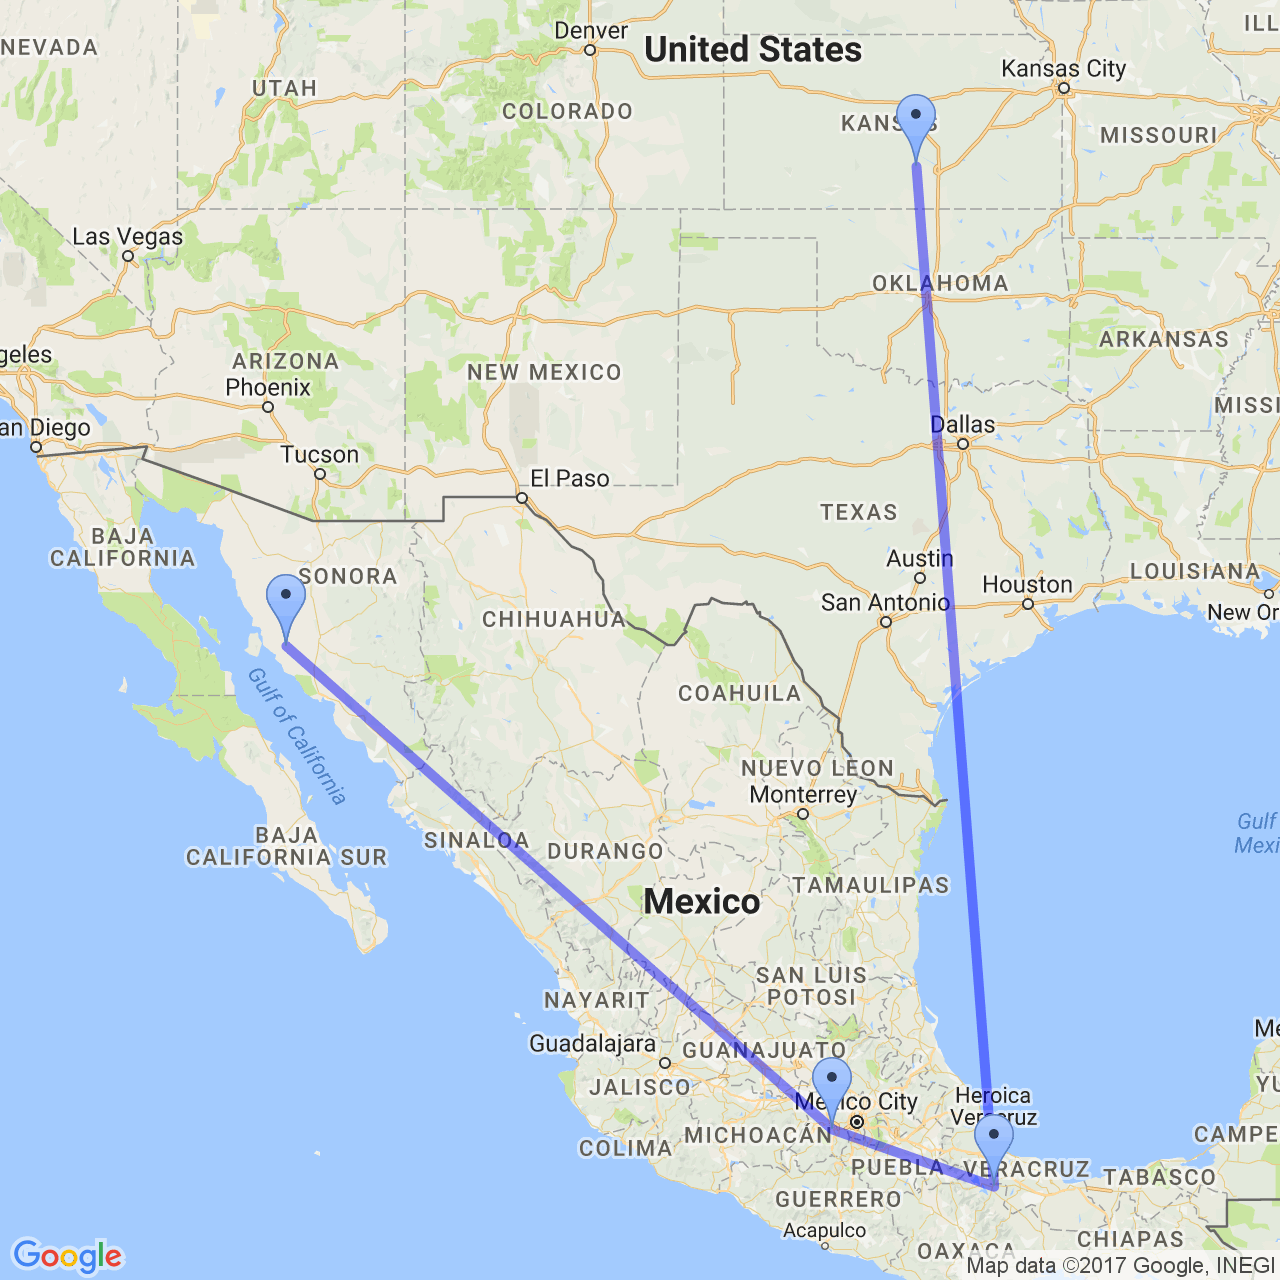
\includegraphics[width=0.55\textwidth]{modules/unam_path_2}
 \label{fig:ruta_unam_2}
\end{figure}
